\documentclass{bioinfo}
\copyrightyear{2010}
\pubyear{2010}

\begin{document}
\begin{application}
\firstpage{1}

\title[SMM Project]{Stabilization matrix method - Mini project}
\author[Sigmar Stefansson, Francesco Favero]{Sigmar Stefansson and Francesco Favero}
\address{Danmarks Tekniske Univeristet}

\history{22 October 2010}

\editor{Supervisor: Morten Nielsen}

\maketitle

\begin{abstract}

\section{Summary}
\textit{RmiR} is an R package for the analysis of microRNA and gene expression microarrays. The goal of this package is to couple microRNA and gene expression data (coming from the same RNA) matching miRNAs to corresponding gene targets using the criteria applied by different databases.
\par The R environment and the bioconductor project allow a complete access to the annotation of a considerable number of microarray chips. \textit{RmiR} also provide a simple way to obtain data trough the standard R way to manage matrix and tables, as well as easy to interpret graphic outputs in SVG format.
\par For series of data, \textit{RmiR} computes the correlation (\cite{ambs2008}) between miRNA and target genes, and gives the most correlated and anti-correlated results, as well as the gene targets which are supposed to be more affected by the microRNA regulation. Moreover for a desired miRNA it is possible to compute the correlations between the miRNA and the global set of genes, not just taking into consideration predicted targets only.

\end{abstract}

\section*{background}

Recently, microRNAs has gained the centre of the scientific scene, the improvement of the molecular technology has increased and played up the importance of these small sequences of nucleotides. As consequence new microRNAs were sent to the miRNA registry from many different scientists and the population of the mature microRNA database (\cite{mirbase2006}) has decisively grown in the latest years.  
\par The interactions that are driven from the regulation of a single miRNA or a few number of them are surprising. Anyway it is not possible to simplify the mechanisms that are involved into such processes by rules. The number of criteria to take into account is so huge to required a computation approach.
\par MicroRNA target prediction is an open field in bioinformatics; many algorithms are developed from different groups over the world. It is somehow true that some miRNA target databases are considered better than others; however, if a target is predicted from any of the prediction algorithms, just an experimental evidence should confirm or deny such hypothesis.
\par For this reason \textit{RmiR} is designed to allow the user to decide which database to use and also to consider results from the intersection of many databases.
\par The possibility of coupling microRNA and gene expression is a captivating research topic. A consistent quantity of data is already available from microarray gene expression and miRNA expression, and a concentration of knowledge to merge the two pieces of biological information should surely lead to a more clear or even different point of view.



\section*{Implementation}

\section*{Description}

The program consist in two different packages; \textit{RmiR}, which includes all the functions to manage the data, and \textit{RmiR.Hs.miRNA} which contains the human miRNA targets databases.
\par To run the program it required at least an input file both for miRNA and gene expression. Obviously, the data of miRNA and gene expression experiments must derive from the same sample or better the same RNA. The file must be formatted to have two columns, the first with the miRNA or the gene identifier and the second with the expression value (e.g. log-ratio, fold change etc.). For gene identifiers a number of different annotations is supported, for microRNA the mature miRNA name is required. 
\par Once imported the data, the function \textit{read.mir} included in \textit{RmiR}, merges the input file in an object containing the transformed data, following the criteria of a single database or the intersection of the selected databases.
\par The object can be inspected by exporting the desired columns in a table or creating an SVG image with the \textit{plotRmiRtc} function. The plot points have the miRNA ad the gene targets expression as coordinates. Each point will contain the annotation information, hidden by default but visible by passing the mouse over the point.

\begin{table}[ht]
\begin{center}
\begin{tabular}{rrlrlr}
  \hline
gene\_id & symbol & geneExpr & mature\_miRNA & mirExpr \\ 
  \hline
286 & ANK1 & -1.41 & hsa-miR-138 & 0.83 \\ 
286 & ANK1 & -1.41 & hsa-miR-27a & -1.15 \\ 
286 & ANK1 & -1.41 & hsa-miR-27b & -2.23 \\ 
351 & APP & -1.67 & hsa-miR-101 & -0.06 \\ 
351 & APP & -1.67 & hsa-miR-20b & 1.61 \\ 
351 & APP & -1.67 & hsa-miR-93 & 1.19 \\ 
351 & APP & -1.67 & hsa-miR-106b & 1.16 \\ 
351 & APP & -1.67 & hsa-miR-20a & 2.12 \\ 
7436 & VLDLR & -1.77 & hsa-miR-20a & 2.12 \\ 
7436 & VLDLR & -1.77 & hsa-miR-20b & 1.61 \\ 
7436 & VLDLR & -1.77 & hsa-miR-106b & 1.16 \\ 
7436 & VLDLR & -1.77 & hsa-miR-93 & 1.19 \\ 
201161 & CENPV & 3.21 & hsa-miR-22 & -2.21 \\ 
   \hline
\end{tabular}
\end{center}
\end{table}

\par The package is better suited to handle series of object created with the function \textit{read.mir} (relative to a time course experiment, for example). In those cases other functions provide the computation of the correlation between the trends of microRNA and relative gene targets expression. Then it is possible to fix a threshold and pick up the most correlated or anti-correlated couples. At the same time, by choice,  a list of genes or microRNAs with the number of miRNA or the number of target, respectively, is generated. These lists are used to highlight the genes or the miRNAs which are possibly more significant and important in the system. The function \textit{plotRmiRtc} provides a plot of the trends of the anti/correlated couples by choosing a gene or a miRNA (figure \ref{fig:01}). If the SVG option is selected, the image will contain hyperlinks to microrna.sanger.ac.uk and http://www.ncbi.nlm.nih.gov to provide information about the microRNAs and the genes.

\begin{figure}[!tpb]
\centerline{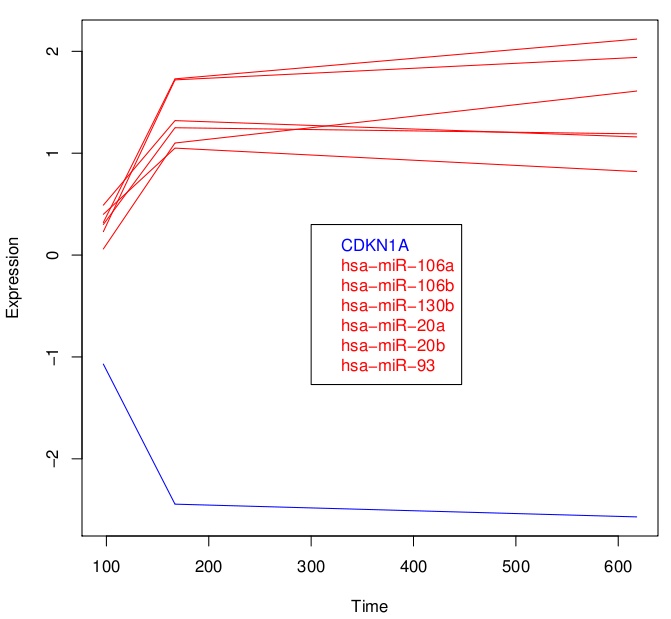
\includegraphics[width=9cm]{cdkn1a.png}}
\caption{Example of result for a RmiR time course experiment}\label{fig:01}
\end{figure}

\par It is not generally true that a target is down regulated when the microRNA is over expressed. So the high correlation ( or anti-correlation ) is not a necessary condition to reveal a relevant relationship. For this reason, with this tool we do not claim to observe all the interactions between miRNAs and mRNAs, but we highlight interesting predicted pairs that need experimental validation. At the same time, if we do not restrict the correlation analysis to predicted pairs, new unpredicted pairs could come up. This could be the case of a gene promoter control by the miRNA, which explains the strong (anti)-correlation found at transcriptional level.






\section*{Acknowledgement}
This work was partially founded by an I.S.I. Foundation grant and by the "Edo Tempia" Foundation.


%\bibliographystyle{natbib}
%\bibliographystyle{achemnat}
%\bibliographystyle{plainnat}
%\bibliographystyle{abbrv}
%\bibliographystyle{bioinformatics}

\bibliographystyle{natbib}

\bibliography{algo}


\end{application}
\end{document}
